	\chapter{}
\label{lecture5}
\section[Квадратичный функционал. Оператор Штурма (Продолжение). ]{Квадратичный функционал. Оператор Штурма--Лиувилля (Продолжение).}
\label{lecture5section1}
Возвращаемся к оператору Штурма с переменными коэффициентами
\begin{equation}
	\label{l5:eq:1}
	\hfill \LL{}y=-\der{}{x}\Big(Q\cdot y'\Big)+P\cdot y\hfill
\end{equation}
в области 
\begin{equation*}
	\hfill\mc{D}_{\LL}=\left\{y(x)|y\in\Cfn[{[a,b]}]{2},\ y(a)=y(b)=0\right\}_{\displaystyle.}\hfill
\end{equation*}
Оператор $\LL$ будем рассматривать в пространстве $\fL[{[a,b]}]$.
\begin{equation*}
	\hfill \fL\eqdef\left\{y(x)\middle|\int\limits_a^b|y(x)|^2\,dx<+\infty\right\}_{\displaystyle.}\hfill
\end{equation*}
Пространство \fL\ состоит из функций, которые интегрируемы с квадратом в смысле Лебега, мы же рассматриваем только функции интегрируемые по Риману как вас учили.\footnote[1]{Заметим, что если функция интегрируема по Риману, то она интегрируема и по Лебегу и оба интеграла совпадают.}

В \fL\ введём скалярное произведение: при $y(x),\,z(x)\in\fL$
\begin{equation*}
	\hfill(y,z)\eqdef\int\limits_a^b y(x)\cdot \overline{z}(x)\,dx\hfill
\end{equation*}  
и норму
\begin{equation*}
	\hfill\norm{y}\eqdef\sqrt{\int\limits_a^b|y(x)|^2\,dx}.\hfill
\end{equation*}
\begin{_def}
	Под \textbf{сходимостью} $z_{m}\to z$ в \fL\ мы будем понимать сходимость по норме
	\begin{equation*}
		\hfill\norm{z_m-z}\to0,\quad m\to\infty.\hfill
	\end{equation*}
\end{_def}

Данная сходимость называется сходимостью в среднем или --- среднеквадратичном. Действительно, пусть $\Delta x=\frac{b-a}{n}$ и $x_i\in i^{\text{ому}}$ отрезку $\Delta x$
\vspace{0,2cm}

\tikzset{every picture/.style={line width=0.75pt}} %set default line width to 0.75pt        

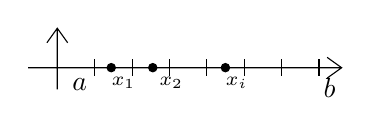
\begin{tikzpicture}[x=0.75pt,y=0.75pt,yscale=-1,xscale=1]
	%uncomment if require: \path (0,50); %set diagram left start at 0, and has height of 50
	
	%Shape: Axis 2D [id:dp9913963713706713] 
	\draw  (57,22.03) -- (208,22.03)(71,3) -- (71,32.5) (201,17.03) -- (208,22.03) -- (201,27.03) (66,10) -- (71,3) -- (76,10)  ;
	%Straight Lines [id:da37737060961638846] 
	\draw    (71.1,22) -- (205,22) (89.1,18) -- (89.1,26)(107.1,18) -- (107.1,26)(125.1,18) -- (125.1,26)(143.1,18) -- (143.1,26)(161.1,18) -- (161.1,26)(179.1,18) -- (179.1,26)(197.1,18) -- (197.1,26) ;
	%Flowchart: Connector [id:dp30749866171285856] 
	\draw  [fill={rgb, 255:red, 0; green, 0; blue, 0 }  ,fill opacity=1 ] (115,22) .. controls (115,20.9) and (115.9,20) .. (117,20) .. controls (118.1,20) and (119,20.9) .. (119,22) .. controls (119,23.1) and (118.1,24) .. (117,24) .. controls (115.9,24) and (115,23.1) .. (115,22) -- cycle ;
	%Flowchart: Connector [id:dp0707282736294279] 
	\draw  [fill={rgb, 255:red, 0; green, 0; blue, 0 }  ,fill opacity=1 ] (95,22) .. controls (95,20.9) and (95.9,20) .. (97,20) .. controls (98.1,20) and (99,20.9) .. (99,22) .. controls (99,23.1) and (98.1,24) .. (97,24) .. controls (95.9,24) and (95,23.1) .. (95,22) -- cycle ;
	%Flowchart: Connector [id:dp7762000733956376] 
	\draw  [fill={rgb, 255:red, 0; green, 0; blue, 0 }  ,fill opacity=1 ] (150,22) .. controls (150,20.9) and (150.9,20) .. (152,20) .. controls (153.1,20) and (154,20.9) .. (154,22) .. controls (154,23.1) and (153.1,24) .. (152,24) .. controls (150.9,24) and (150,23.1) .. (150,22) -- cycle ;
	
	% Text Node
	\draw (77,25.9) node [anchor=north west][inner sep=0.75pt]    {$a$};
	% Text Node
	\draw (198,25.9) node [anchor=north west][inner sep=0.75pt]    {$b$};
	% Text Node
	\draw (119,25.4) node [anchor=north west][inner sep=0.75pt]  [font=\scriptsize]  {$x_{2}$};
	% Text Node
	\draw (96,25.4) node [anchor=north west][inner sep=0.75pt]  [font=\scriptsize]  {$x_{1}$};
	% Text Node
	\draw (151,25.4) node [anchor=north west][inner sep=0.75pt]  [font=\scriptsize]  {$x_{i}$};
	
	
\end{tikzpicture}

\begin{equation*}
	\norm{z_m-z}=\sqrt{\int\limits_a^b\big|z_m(x)-z(x)\big|^2\,dx}=\sqrt{\lim\limits_{n\to\infty}\sum\limits_{i=1}^n\frac{\big|z_m(x_i)-z(x_i)\big|^2}{n}\cdot(b-a)},
\end{equation*}
а это и есть среднее с точностью до множителя $\sqrt{b-a}$.

Зачем нужно пространство \fL[(a,b)]? В курсе линейной алгебры мы изучали линейные операторы в пространствах со скалярным произведением и выделили некоторые классы операторов, обладающих важными свойствами. Для нас будут важны симметричные (эрмитовы) операторы $A$, для которых
\begin{equation*}
	\hfill (Ay,z)=(y,Az)\quad\text{при }y,\,z\in\mc{D}_{\!A}\text{ --- область определения }A.\hfill 
\end{equation*} 
Мы покажем далее, что оператор Штурма --- эрмитов.

Есть ещё одно преимущество рассмотрения пространства \fL[(a,b)]{}: это сходимость. 
\begin{_def}
	Если $z_m(x)$ --- последовательность непрерывных функций, то говорят, что она \textbf{сходится равномерно} к функции $z(x)$ если
	\begin{equation*}
		\hfill\sup\limits_{x\in[a,b]}|z_m(x)-z(x)|\to0\quad\text{ при }m\to\infty.\hfill
	\end{equation*}
\end{_def}   
\begin{_def}
	\textbf{Расстояние между функциями }в равномерной метрике --- это
	\begin{equation*}
		\hfill\sup\limits_{x\in[a,b]}|z_m(x)-z(x)|.\hfill
	\end{equation*}
\end{_def}
Например, пусть $[a,b]=[0,1]$\ и\  \parbox[t]{0,18\textwidth}{
	$\begin{array}{ll}
		z=1&x\in[0,1]\\
		z_m=0&x\in[0,1]
	\end{array}$} тогда 
\parbox[c]{0,25\textwidth}{\fbox{$\sup\limits_{x\in[0,1]}|z_m(x)-z(x)|=1$}}.

\tikzset{every picture/.style={line width=0.75pt}} %set default line width to 0.75pt        

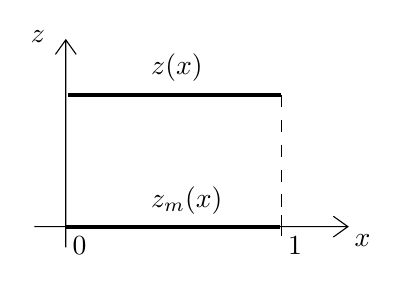
\begin{tikzpicture}[x=0.75pt,y=0.75pt,yscale=-1,xscale=1]
	%uncomment if require: \path (0,142); %set diagram left start at 0, and has height of 142
	
	%Shape: Axis 2D [id:dp8517287319738365] 
	\draw  (57,105) -- (208,105)(72.1,15) -- (72.1,115) (201,100) -- (208,105) -- (201,110) (67.1,22) -- (72.1,15) -- (77.1,22)  ;
	%Straight Lines [id:da340068278357303] 
	\draw    (176,99.5) -- (176,109.5) ;
	%Straight Lines [id:da28165501951031624] 
	\draw  [dash pattern={on 4.5pt off 4.5pt}]  (176,41.5) -- (176,98.5) ;
	%Straight Lines [id:da5695980520276169] 
	\draw [line width=1.5]    (73,41.5) -- (176,41.5) ;
	%Straight Lines [id:da6011126376651919] 
	\draw [line width=1.5]    (72.1,105) -- (175.1,105) ;
	
	% Text Node
	\draw (210,107.4) node [anchor=north west][inner sep=0.75pt]    {$x$};
	% Text Node
	\draw (54,9.4) node [anchor=north west][inner sep=0.75pt]    {$z$};
	% Text Node
	\draw (74.1,108.4) node [anchor=north west][inner sep=0.75pt]    {$0$};
	% Text Node
	\draw (178,108.4) node [anchor=north west][inner sep=0.75pt]    {$1$};
	% Text Node
	\draw (112,20.4) node [anchor=north west][inner sep=0.75pt]    {$z( x)$};
	% Text Node
	\draw (112,84.4) node [anchor=north west][inner sep=0.75pt]    {$z_{m}( x)$};
	
	
\end{tikzpicture}

Пусть \parbox[t]{0,26\textwidth}{
	$\displaystyle \tilde{z}_m=\begin{cases}
		m\cdot x&0\leqslant x\leqslant \frac{1}{m}\\
		1&\!\frac{1}{m}\leqslant x\leqslant 1
	\end{cases}$} $\Rightarrow$ \parbox[t]{0,33\textwidth}{
	$\displaystyle z-\tilde{z}_m=\begin{cases}
		1-m\cdot x&0\leqslant x\leqslant \frac{1}{m}\\
		0&\!\frac{1}{m}\leqslant x\leqslant 1
	\end{cases}$} и \parbox[c]{0,25\textwidth}{\fbox{$\sup\limits_{x\in[0,1]}|\tilde{z}_m(x)-z(x)|=1$}}.

\tikzset{every picture/.style={line width=0.75pt}} %set default line width to 0.75pt        

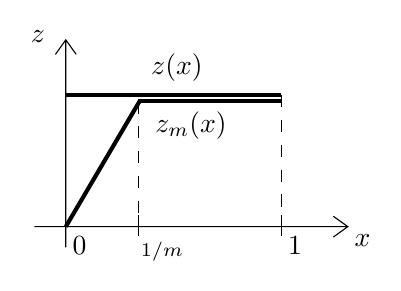
\begin{tikzpicture}[x=0.75pt,y=0.75pt,yscale=-1,xscale=1]
	%uncomment if require: \path (0,142); %set diagram left start at 0, and has height of 142
	
	%Shape: Axis 2D [id:dp7975069141949729] 
	\draw  (57,105) -- (208,105)(72.1,15) -- (72.1,115) (201,100) -- (208,105) -- (201,110) (67.1,22) -- (72.1,15) -- (77.1,22)  ;
	%Straight Lines [id:da054186325683345915] 
	\draw    (176,99.5) -- (176,109.5) ;
	%Straight Lines [id:da006975025053542305] 
	\draw  [dash pattern={on 4.5pt off 4.5pt}]  (176,41.5) -- (176,98.5) ;
	%Straight Lines [id:da8077397061828984] 
	\draw [color={rgb, 255:red, 0; green, 0; blue, 0 }  ,draw opacity=1 ][line width=1.5]    (72,41.5) -- (176,41.5) ;
	%Straight Lines [id:da9931878510195675] 
	\draw [line width=1.5]    (108,44) -- (72.1,105) ;
	%Straight Lines [id:da8497979609998774] 
	\draw [line width=1.5]    (107,44.5) -- (176,44.5) ;
	%Straight Lines [id:da8990171803302427] 
	\draw    (107,99.5) -- (107,109.5) ;
	%Straight Lines [id:da9524229647340969] 
	\draw  [dash pattern={on 4.5pt off 4.5pt}]  (107,44.5) -- (107,101.5) ;
	
	% Text Node
	\draw (210,107.4) node [anchor=north west][inner sep=0.75pt]    {$x$};
	% Text Node
	\draw (54,9.4) node [anchor=north west][inner sep=0.75pt]    {$z$};
	% Text Node
	\draw (74.1,108.4) node [anchor=north west][inner sep=0.75pt]    {$0$};
	% Text Node
	\draw (178,108.4) node [anchor=north west][inner sep=0.75pt]    {$1$};
	% Text Node
	\draw (112,20.4) node [anchor=north west][inner sep=0.75pt]    {$z( x)$};
	% Text Node
	\draw (114,48.4) node [anchor=north west][inner sep=0.75pt]    {$z_{m}( x)$};
	% Text Node
	\draw (107,110.9) node [anchor=north west][inner sep=0.75pt]  [font=\scriptsize]  {$1/m$};
	
\end{tikzpicture}

\noindent Сравним две последовательности $z_m$ и $\tilde{z}_m$. \parbox[с]{0,55\textwidth}{$z_m-z$=1 во всех точках\\
	$\tilde{z}_m-z$=1 только при $x=0$, а при $1\bigm/m\leqslant x\leqslant1$ $\tilde{z}=z$.}
Но метрика $\sup\limits_{x\in[0,1]}|\tilde{z}_m(x)-z(x)|$ этого не чувствует, хотя при $m\to\infty$ интервал совпадений функций $\tilde{z}_m$ и $z$ стремится ко всему интервалу! В тоже время $\norm{z_m-z}=1$, а 
\begin{equation*}
	\hfill{\norm{\tilde{z}_m-z}}^2=\int\limits_{0}^{1\bigm/m}(m\cdot x-1)^2\,dx\to0,\hfill
\end{equation*}					
то есть метрика в \fL\ <<чувствует>> ситуацию и описывает её более точно.

\noindent Вернёмся теперь к оператору $\LL$. Докажем, что оператор \LL\ --- эрмитов в $\mc{D}_{\LL}$. Пусть $y(x),\,z(x)\in\mc{D}_{\LL}$. Тогда
\begin{equation*}
	\big(\LL y,z\big)=\int\limits_a^b \underbrace{\overline{z}}_{v}\cdot\underbrace{\left(-\der{}{x}\Big(Q\cdot y'\Big)\right)\,dx}_{du}+\int\limits_a^b P\cdot y\cdot\overline{z}\,dx=-Q\cdot y'\cdot\overline{z}\mathop{\Big|}\limits_a^b+\int\limits_a^b\left(Q\cdot y'\cdot\overline{z}'+P\cdot y\cdot\overline{z}\right)\,dx.
\end{equation*}
Так как $z(a)=z(b)=0$, то в итоге 
\begin{equation}
	\label{l5:eq:2}
	\hfill\big(\LL y,z\big)=\int\limits_a^b\left(Q\cdot y'\cdot\overline{z}'+P\cdot y\cdot\overline{z}\right)\,dx.\hfill
\end{equation}
Далее $\big(y,\LL z\big)=\overline{\big(\LL z,y\big)}$. Значит для получения $\big(y,\LL z\big)$ надо в~\eqref{l5:eq:2} $y\leftrightarrow z$ и взять комплексное сопряжение. Если это сделать, то окажется, что
\begin{equation*}
	\hfill\big(\LL y,z\big)=\big(y,\LL z\big),\hfill
\end{equation*} 
то есть оператор \LL\ --- эрмитов. Отсюда следует, что его собственные значения вещественны. Действительно, пусть $\LL y=\lambda\cdot y$. Умножим на $y$ скалярно обе части. Получим
\begin{equation*}
	\hfill\big(\LL y,y\big)=\lambda\cdot{\norm{y}}^2,\hfill
\end{equation*}
но $\big(\LL y,y\big)=\big(y,\LL y\big)$ --- в силу эрмитовости, а $\big(y,\LL y\big)=\overline{\big(\LL y,y\big)}$. Значит $\big(\LL y,y\big)$ --- вещественно, то есть $\lambda$ --- вещественно. Кстати, это можно было получить из~\eqref{l5:eq:2}, полагая там $z=y$:
\begin{equation}
	\label{l5:eq:3}
	\hfill \big(\LL y,y\big)=\int\limits_a^b\left(Q\cdot|y'|^2+P\cdot|y|^2\right)\,dx=\J[y].\hfill
\end{equation}
(Конечно $\big(\LL y,y\big)=\J[y]$ --- для вещественных $y$)

Так как $\lambda$ --- вещественно, то собственные функции оператора \LL\ можно считать вещественными, ибо если $y=\Re y+i\cdot\Im y$, то 
\begin{equation*}
	\hfill\LL\left(\Re y+i\cdot\Im y\right)=\lambda\cdot\left(\Re y+i\cdot\Im y\right)\hfill
\end{equation*} 
и значит 
\begin{equation*}
	\hfill\LL\,\Im y=\lambda\cdot\Im y,\quad\LL\Re y=\lambda\cdot\Re y.\hfill
\end{equation*}

Далее, собственные функции оператора \LL, отвечающие его различным собственным значениям, взаимно ортогональны. Докажем это. Имеем
\begin{equation*}
	\hfill\LL y=\lambda\cdot y,\quad\LL z=\nu\cdot z,\quad y,\,z\in\mc{D}_{\LL},\quad \lambda\neq\nu.\hfill
\end{equation*}   
Тогда 
\begin{equation}
	\label{l5:eq:4}
	\hfill \big(y,z\big)=0.\hfill
\end{equation}
Действительно, умножим равенство $\LL y=\lambda\cdot y$ на $z$ скалярно. Получим
\begin{equation*}
	\hfill\big(\LL y,z\big)=\lambda\cdot\big(y,z\big),\hfill
\end{equation*}
но
\begin{equation*}
	\quad\big(\LL y,z\big)=\big(y,\LL z\big)=\big(y,\nu\cdot z\big)=\nu\cdot\big(y,\,z\big)\quad\text{(напомним, что $\nu$ --- вещественно).}
\end{equation*}
Таким образом
\begin{equation*}
	\big(\LL y,z\big)=\nu\cdot\big(y,z\big)=\lambda\cdot\big(y,z\big)\quad\Rightarrow\quad \big(\nu-\lambda\big)\cdot \big(y,z\big)=0\quad\Rightarrow\quad\big(y,z\big)=0.
\end{equation*}
То есть~\eqref{l5:eq:4} --- доказано.

Докажем теперь, что собственные подпространства оператора Штурма одномерны (эквивалентная формулировка: собственные значения не вырождены\footnote{Напомним, что мы называем собственное значение $\lambda$ \textbf{вырожденным}, если для собственного подпространства \Ul,\ $\dim\Ul\geqslant2$}.)

Итак, пусть 
\begin{equation}
	\label{l5:eq:5}
	\hfill\LL y=\lambda\cdot y\hfill
\end{equation}
и
\begin{equation*}
	\hfill\Ul=\left\{y(x)|y\in\mc{D}_{\LL},\ Ly=\lambda\cdot y\right\}_{\displaystyle.}\hfill
\end{equation*}
Докажем, что $\dim\Ul=1$. Перепишем равенство~\eqref{l5:eq:5} в виде
\begin{multline}
	\label{l5:eq:5a}
	-\der{}{x}\big(Q\cdot y'\big)+P\cdot y=\lambda\cdot y\quad\Rightarrow\quad-Q\cdot y''-Q'\cdot y'+P\cdot y=\lambda\cdot y\quad\Rightarrow\\\Rightarrow\quad y''+\frac{Q'(x)}{Q(x)}\cdot y'+\frac{\lambda-P}{Q(x)}\cdot y=0,\quad\text{так как $\Ul\subset\mc{D}_{L}$}.
\end{multline}
 Таким образом все собственные функции из собственного подпространства есть решения уравнения~\eqref{l5:eq:5a} с граничными условиями  $y(a)=y(b)=0$.

Пусть $y_1,\,y_2\in\Ul$. Так как оператор \LL\ --- линейный, то любая линейная комбинация
\begin{equation*}
	\hfill y=c_1\cdot y_1+c_2\cdot y_2\in\Ul\hfill
\end{equation*} 
и значит, удовлетворяет~\eqref{l5:eq:5a}. Положим 
\begin{equation*}
	\hfill y(x)\eqdef y_1(x)\cdot y'_2(a)-y_2(x)\cdot y_1'(a).\hfill
\end{equation*}
В силу граничных условий $y_1(a)=y_2(a)=0$ и поэтому $y(a)=0$. Далее
\begin{equation*}
	\hfill y'(x)=y_1'(x)\cdot y'_2(a)-y'_2(x)\cdot y_1'(a).\hfill
\end{equation*}
Очевидно $y'(a)=0$. Таким образом решение $y(x)$ уравнения~\eqref{l5:eq:5a} удовлетворяет условию\\ $y(a)=y'(a)=0$. При $Q(a)\neq0$ в силу теоремы единственности решение $y(x)$ совпадает с решением $y\equiv0$. Таким образом 
\begin{equation}
	\label{l5:eq:6}
	\hfill y_1(x)\cdot y'_2(a)-y_2(x)\cdot y'_1(a)\equiv0.\hfill
\end{equation}
$y'_1(a)\neq0$, ибо иначе $y_1\equiv0$, поскольку $y_1(a)=0$, поэтому из~\eqref{l5:eq:6}
\begin{equation*}
	\hfill y_2(x)=y_1(x)\cdot\frac{y'_2(a)}{y'_1(a)}.\hfill
\end{equation*}  
Следовательно, любые решения~\eqref{l5:eq:5a} (то есть любая функция из \Ul) получается умножением фиксированной функции на подходящую константу. Поэтому $\dim\Ul=1$, что и требовалось доказать.
\begin{_con}
	Нормированная собственная функция, отвечающая данному собственному значению, единственна с точностью до знака.
\end{_con}

\noindent\textbf{Задание. }Доказательство проведено в случае $Q(x)>0$, $x\in[a,b]$, но у нас будет случай: $Q(x)=x$, $[a,b]=[0,R]$. Здесь $Q(a)=0$. Как провести доказательство в этом случае?

\section[Экстремальные свойства собственных значений оператора Штурма.]{Экстремальные свойства собственных значений и собственных функций оператора Штурма.}
\label{lecture5section2}
\begin{multline*}
	\text{Решая задачу на }\min\limits_{y\in\K}\,\J[y],\quad\J[y]=\int\limits_a^b\left(Q\cdot y'^2+P\cdot y^2\right)\,dx\\
	\K=\left\{y(x)|y\in\Cfn[{[a,b]}]{1},\ y(a)=y(b)=0,\ \int\limits_a^b y^2\,dx=1\right\},
\end{multline*}
мы пришли к тому, что минимайзер есть собственная функция оператора Штурма
\begin{equation}
	\label{l5:eq:7}
	\hfill Ly=\lambda\cdot y,\hfill
\end{equation}
где 
\begin{equation*}
	\hfill Ly=-\der{}{x}\big(Q\cdot y'\big)+P\cdot y,\quad\mc{D}_{L}=\left\{y(x)|y\in\Cfn[{[a,b]}]{2},\ y(a)=y(b)=0\right\}_{\displaystyle.}\hfill
\end{equation*}

Рассматривая случаи постоянных коэффициентов $Q(x)=c_1$, $P(x)=c_2$ мы нашли \emph{бесконечную серию} собственных значений $\lambda_k$ и соответствующих собственных функций $y_k$. Естественно возникает вопрос: какое отношение имеют эти собственные значения и собственные функции к функционалу $\J[y]$ и вообще к вариационным задачам? Ответ на этот вопрос дают теоремы~\ref{l5:s2:teor:1}--\ref{l5:s2:teor:3}, которые мы сейчас сформулируем и докажем для оператора Штурма с переменными коэффициентами. Нам удобно в дальнейшем переобозначить класс \K, положив $\K_1\equiv\K$.
\begin{_teor}
	\label{l5:s2:teor:1}
	Минимайзер задачи на $\displaystyle\min\limits_{y\in\K_1}\,\J[y]$ есть собственная функция $y_1(x)$ оператора Штурма, отвечающая его наименьшему собственному значению $\lambda_1$ и $\lambda_1=\J[y_1]$.
\end{_teor}
\begin{_teor}
	\label{l5:s2:teor:2}
	Пусть $\displaystyle\K_2\eqdef\left\{y(x)|y\in\K_1,\ \big(y,y_1\big)=0\right\}$. Тогда минимайзер задачи на $\displaystyle\min\limits_{y\in\K_2}\,\J[y]$ есть собственная функция $y_2(x)$ оператора Штурма отвечающая его второму по величине собственному значению $\lambda_2$ и $\lambda_2=\J[y_2]$.
\end{_teor}
\begin{_teor}
	\label{l5:s2:teor:3}
	Пусть $y_1,y_2,\ldots,y_{p-1}$ --- нормированные собственные функции оператора Штурма, отвечающие его первым $p-1$ (по величине) собственным значениям $\lambda_1,\ldots,\lambda_{p-1}$ и 
	\begin{equation*}
		\hfill\displaystyle\K_p\eqdef\left\{y(x)|y\in\K_1,\ \big(y,y_j\big)=0,\,j=\overline{1,p-1}\right\}_{\displaystyle.}\hfill
	\end{equation*}
	Тогда минимайзер в задаче на $\displaystyle\min\limits_{y\in\K_p}\,\J[y]$ есть собственная функция, отвечающая $p$-ому (по величине) собственному значению $\lambda_p$ оператора Штурма и $\lambda_p=\J[y_p]$.  
\end{_teor}
Переходим к доказательству теорем~\ref{l5:s2:teor:1}--\ref{l5:s2:teor:3}. 	Всюду считаем, что минимайзеры в рассматриваемых задачах существуют (доказательство --- вне нашего курса). 
\begin{proof}[Доказательство теоремы~\ref{l5:s2:teor:1}.]
	
	Пусть $y_1(x)$ --- минимайзер в задаче на $\min\limits_{y\in\K_1}\,\J[y]$. Как мы знаем, тогда 
	\begin{equation*}
		\hfill Ly_1=\lambda\cdot y_1\hfill
	\end{equation*} 
	и $\lambda=\big(Ly_1,y_1\big)=\J[y_1]$. Покажем, что $\lambda$ --- наименьшее собственное значение $\lambda_1$ оператора $L$. Пусть $\nu$ --- произвольное собственное значение оператора $L$ и $z=z(x)$ --- соответствующая собственная функция: $Lz=\nu\cdot z$. Считаем, что $\norm{z}=1$ и тогда $\nu=\big(Lz,z\big)=\J[z]$. Но $z\in\mc{D}_{L}$ и $\norm{z}=1$, поэтому $z\in\K_1$ и значит $\J[z]\geqslant\min\limits_{y\in\K_1}\,\J[y]=\J[y_1]$. Но $\J[y_1]=\lambda$ и значит $\nu\geqslant\lambda$. Таким образом $\lambda$ действительно наименьшее собственное значение $\lambda_1$ оператора Штурма, а $y_1$ --- соответствующая собственная функция.
\end{proof}

\begin{proof}[Доказательство теоремы~\ref{l5:s2:teor:2}.] Пусть 
	\begin{equation*}
		\hfill\K_2=\left\{y(x)|y\in\K_1,\ \big(y,y_1\big)=0\right\},\quad\Big[\K_1=\left\{y(x)|y\in\Cfn[{[a,b]}]{1},\ y(a)=y(b)=0,\ \norm{y}=1\right\}\Big]_{\displaystyle.}\hfill
	\end{equation*} 
	и $y_2$ --- минимайзер в задаче на $\min\limits_{y\in\K_2}\,\J[y]$. Найдём уравнение для $y_2$. Согласно общей теории изопериметрических задач, составляем 
	\begin{equation*}
		\hfill F^{\ast}=F-\lambda\cdot y^2-\mu\cdot y\cdot y_1\hfill
	\end{equation*}
	и пишем уравнение Эйлера 
	\begin{equation*}
		\hfill F^{\ast}_y-\der{}{x}F^{\ast}_{y'}=0\quad\Rightarrow\quad 2\cdot P\cdot y_2-2\cdot\lambda\cdot y_2-\mu\cdot y_1-2\cdot\der{}{x}\big(Q\cdot y'_2\big)=0,\hfill
	\end{equation*}
	где $\lambda$ и $\mu$ --- неизвестные константы. Перепишем это уравнение в виде
	\begin{equation}
		\label{l5:eq:8}
		\hfill Ly_2=\lambda\cdot y_2+\frac{\mu}2\cdot y_1.\hfill
	\end{equation}
	Докажем, что $\mu=0$. Умножим обе части~\eqref{l5:eq:8} на $y_1$ скалярно. Получим
	\begin{equation}
		\label{l5:eq:9}
		\hfill\big(Ly_2,y_1\big)=\lambda\cdot\big(y_2,y_1\big)+\frac{\mu}{2}\cdot \norm{y_1}^2,\hfill
	\end{equation} 
	но $\big(Ly_2,y_1\big)=\big(y_2,Ly_1\big)=\lambda_1\cdot\big(y_2,y_1\big)$. Поскольку $y_2\in\K_2$, то $\big(y_2,y_1\big)=0$ поэтому в~\eqref{l5:eq:9}
	\begin{equation*}
		\hfill 0,5\cdot\mu\cdot\norm{y_1}^2=0\quad\Rightarrow\quad\mu=0.\hfill
	\end{equation*}
	Следовательно~\eqref{l5:eq:8} переходит в 
	\begin{equation*}
		\hfill Ly_2=\lambda\cdot y_2,\hfill
	\end{equation*}
	где $\lambda=\big(Ly_2,y_2\big)=\J[y_2]$. Остаётся доказать, что $\lambda$ --- второе по величине собственное значение оператора Штурма. Пусть $\nu$ --- произвольное собственное значение оператора Штурма $\nu>\lambda_1$, и $z(x)$ --- соответствующая нормированная собственная функция. Имеем 
	\begin{equation*}
		\hfill Lz=\nu\cdot z.\hfill
	\end{equation*}
	Откуда $\big(Lz,z\big)=\J[z]=\nu$. Так как $z\in\mc{D}_{L}$, то $z\in\Cfn[{[a,b]}]{2}$, $z(a)=z(b)=0$. Кроме того, поскольку $\nu\neq\lambda_1$, то в силу взаимной ортогональности собственных функций отвечающих \emph{различным} собственным значениям оператора $L$ выполняется $\big(z,y_1\big)=0$. Из вышесказанного вытекает, что $z\in\K_2$ и, следовательно,
	\begin{equation*}
		\hfill\nu=\J[z]\geqslant\J[y_2]=\lambda.\hfill
	\end{equation*} 
	Следовательно $\lambda$ является вторым по величине собственным значением $\lambda_2$ оператора Штурма. \emph{Теорема~\ref{l5:s2:teor:2} доказана}. 
\end{proof}
\begin{proof}[Доказательство теоремы~\ref{l5:s2:teor:3}.]
	Пусть $\lambda_1<\lambda_2<\ldots<\lambda_{p-1}$ --- первые $(p-1)$ собственные значения оператора Штурма и $y_1,\ y_2,\ldots,y_{p-1}$ --- соответствующие нормированные собственные функции,
	\begin{equation*}
		\hfill\K_{p}=\left\{y(x)|y\in\K_1,\  \big(y,y_j\big)=0,\,j=\overline{1,p-1}\right\}_{\displaystyle.}\hfill
	\end{equation*}
	Докажем, что минимайзер $y_p$ задачи на $\min\limits_{y\in\K_p}\,\J[y]$ есть собственная функция оператора $L$, отвечающая его $p$-ому по величине собственному значению $\lambda_p$. Для доказательства запишем уравнение для $y_p$. Согласно теории изопериметрических задач составляем
	\begin{gather*}
		F^{\ast}=Q\cdot y^{\prime2}+P\cdot y^2-\lambda\cdot y^2-\sum\limits_{j=1}^{p-1}\mu_j\cdot y_j\cdot y\quad\text{и пишем уравнение для }y_p\\
		2\cdot P\cdot y_p-2\cdot\lambda_p=\sum\limits_{j=1}^{p-1}\mu_j\cdot y_j-2\cdot\der{}{x}\big(Q\cdot y'_p\big)=0,\quad\text{откуда}
	\end{gather*}  
	\begin{equation}
		\label{l5:eq:10}
		\hfill Ly_p=-\der{}{x}\big(Q\cdot y'_p\big)+P\cdot y_p=\lambda\cdot y_p+\sum\limits_{j=1}^{p-1}\frac{\mu_j\cdot y_j}{2}.\hfill
	\end{equation}
	Как и в теореме~\ref{l5:s2:teor:2} покажем, что $\mu_j=0,\,j=\overline{1,p-1}$. Для этого домножим обе части~\eqref{l5:eq:10} на $y_i$ скалярно. Тогда получим
	\begin{equation}
		\label{l5:eq:11}
		\hfill\big(Ly_p,y_i\big)=\lambda\cdot\big(y_p,y_i\big)+\frac12\cdot\sum\limits_{j=1}^{p-1}\mu_j\cdot\big(y_j,y_i\big).\hfill
	\end{equation}
	Как мы знаем $\big(y_j,y_i\big)=\delta_{ij}$. Кроме того 
	\begin{equation*}
		\hfill\big(Ly_p,y_i\big)=\big(y_p,\lambda_i\cdot y_i\big)=\lambda_i\cdot\big(y_p,y_i\big)=0,\hfill
	\end{equation*}
	при $i\leqslant p-1$ по определению класса $\K_p$. Учитывая сказанное, получим в~\eqref{l5:eq:11}
	\begin{equation*}
		\hfill0=0+\frac12\cdot\sum\limits_{j=1}^{p-1}\mu_j\cdot\delta_{ij}=\frac{\mu_i}{2},\quad\forall i, 1\leqslant i\leqslant p-1.\hfill
	\end{equation*}
	Поэтому уравнение~\eqref{l5:eq:10} примет вид $Ly_p=\lambda\cdot y_p$ и нам остаётся доказать, что $\lambda=\lambda_p$. 
	
	Очевидно, $\J[y_p]=\lambda$ и $\lambda_j\neq\lambda,\,j=\overline{1,p-1}$, ибо иначе собственному значению $\lambda_j$ отвечали бы две взаимно ортогональные функции $y_j$ и $y_p$, это невозможно, ибо $\dim\Ul[\lambda_j]=1$, а $y_j$ и $y_p$ --- линейно не зависимы. Пусть $\nu$ --- любое собственное значение оператора $L$, не совпадающее с $\lambda_1,\,\lambda_2,\ldots,\lambda_{p-1}$. Покажем, что $\nu\geqslant\lambda$. Пусть $z(x)$ --- нормированная собственная функция, отвечающая $\nu$. Тогда 
	\begin{equation*}
		\hfill Lz=\nu\cdot z\quad\Rightarrow\quad\big(Lz,z\big)=\J[z]=\nu.\hfill
	\end{equation*} 
	Так как $\nu\neq\lambda_1,\ldots,\lambda_{p-1}$, то $\big(z,y_j\big)=0,\,j=\overline{1,p-1}$, поэтому $z\in\K_p$ и, значит,
	\begin{equation*}
		\hfill\J[z]\geqslant\min\limits_{y\in\K_p}\,\J[y]=\J[y_p]=\lambda.\hfill
	\end{equation*} 
	Значит $\nu\geqslant\lambda$, то есть $\lambda$ --- действительно $p$-ое по величине собственное значение $\lambda_p$ оператора $L$. \emph{Теорема~\ref{l5:s2:teor:3} доказана}. 
\end{proof}

Наряду с этими теоремами существует ещё одна, которая позволяет описать $p$-ое собственное значение оператора Штурма с помощью решения некоторых вариационных задач без знания собственных функций, отвечающих первым $p-1$ собственным значениям.
\begin{_teor}[принцип минимакса]
	\label{l5:s2:teor:4}
	Пусть как и раньше $\lambda_1<\lambda_2<\ldots<\lambda_{p-1}$ первые $(p-1)$ собственные значения оператора Штурма и $y_1,\,y_2,\ldots,y_{p-1}$ --- соответствующие нормированные собственные функции, а $\phi_1,\ldots,\phi_{p-1}$ --- произвольные функции из $\fL$. Теорема утверждает, что
	\begin{equation}
		\label{l5:eq:12}
		\hfill\lambda_p=\max\limits_{\phi_1,\ldots,\phi_{p-1}}\quad\min\limits_{\substack{y\in\K,\\\lefteqn{\scriptstyle \hspace*{-0.8cm}y\perp\phi_1,\phi_2,\ldots,\phi_{p-1}}}}\,J[y].\hfill
	\end{equation}
\end{_teor}
\begin{proof}
	Для фиксированного набора $\phi_1,\ldots,\phi_{p-1}$ положим
	\begin{equation}
		\label{l5:eq:13}
		\hfill\nu(\phi_1,\ldots,\phi_{p-1})\eqdef\min\limits_{\substack{y\in\K,\\\lefteqn{\scriptstyle \hspace*{-0.8cm}y\perp\phi_1,\phi_2,\ldots,\phi_{p-1}}}}\,J[y],\hfill
	\end{equation}
	тогда~\eqref{l5:eq:12} означает, что
	\begin{equation}
		\label{l5:eq:14}
		\hfill\lambda_p=\max\limits_{\phi_1,\ldots,\phi_{p-1}}\nu(\phi_1,\ldots,\phi_{p-1}).\hfill
	\end{equation}
	Положим $\displaystyle\alpha\eqdef\max\limits_{\phi_1,\ldots,\phi_{p-1}}\nu(\phi_1,\ldots,\phi_{p-1})$. Нам надо установить, что $\alpha=\lambda_p$. В силу теоремы~\ref{l5:s2:teor:3} $\nu(y_1,\ldots,y_{p-1})=\lambda_p$ и значит $\alpha\geqslant\lambda_p$. Остаётся показать, что
	\begin{equation}
		\label{l5:eq:15}
		\hfill\alpha\leqslant\lambda_p.\hfill
	\end{equation} 
	Для доказательства~\eqref{l5:eq:15} мы покажем, что $\nu(\phi_1,\ldots,\phi_{p-1})\leqslant\lambda_p$ при $\forall\phi_1,\ldots,\phi_{p-1}$. А так как $\alpha=\max\limits_{\phi_1,\ldots,\phi_{p-1}}\nu(\phi_1,\ldots,\phi_{p-1})$, то тогда $\alpha\leqslant\lambda_p$.
	
	Итак, пусть $\phi_1,\ldots,\phi_{p-1}$ --- любой набор из $\fL$ и мы докажем, что
	\begin{equation}
		\label{l5:eq:16}
		\hfill\nu(\phi_1,\ldots,\phi_{p-1})\leqslant\lambda_p.\hfill
	\end{equation}  
	Рассмотрим 
	\begin{equation*}
		\hfill \tilde{y}_0=\sum\limits_{j=1}^{p}\tilde{c}_j\cdot y_j\hfill
	\end{equation*}
	и подберём коэффициенты $\tilde{c}_j$ так, чтобы $\big(\tilde{y},\phi_i\big)=0,\,i=\overline{1,p-1}$. Чтобы эти равенства выполнялись, очевидно, числа $\tilde{c}_j$ должны удовлетворять условиям
	\begin{equation}
		\label{l5:eq:17}
		\hfill \sum\limits_{j=1}^{p}\tilde{c}_j\cdot \big(y_j,\phi_i\big)=0,\quad i=\overline{1,p-1}.\hfill
	\end{equation} 
	\eqref{l5:eq:17} --- система $(p-1)$ однородных уравнений относительно $p$ неизвестных $\tilde{c}_1,\ldots,\tilde{c}_p$. Так как число неизвестных больше числа уравнений, то существует не нулевое решение $\tilde{c}_1,\ldots,\tilde{c}_p$. Так как решение~\eqref{l5:eq:17} определено с точностью до произвольного множителя, то числа 
	\begin{equation*}
		\hfill c_j\eqdef\frac{\tilde{c}_j}{\sqrt{\sum\limits_{i=1}^p|\tilde{c}_i|^2}},\quad j=\overline{1,p}.\hfill
	\end{equation*}
	тоже будут решением~\eqref{l5:eq:17} и поэтому функция $\displaystyle y_0=\sum\limits_{j=1}^{p}c_j\cdot y_j$ ортогональна к $\phi_1,\ldots,\phi_{p-1}$. Кроме того
	\begin{equation*}
		\hfill\big(y_0,y_0\big)=\left(\sum\limits_{j=1}^{p}c_j\cdot y_j,\sum\limits_{s=1}^{p}c_s\cdot y_s\right)=\sum\limits_{s=1}^p|c_s|^2=1.\hfill
	\end{equation*}
	Очевидно, что $y_0(x)\in\K$, поэтому
	\begin{equation}
		\label{l5:eq:18}
		\hfill\nu(\phi_1,\ldots,\phi_{p-1})=\min\limits_{\substack{y\in\K,\\\lefteqn{\scriptstyle \hspace*{-0.8cm}y\perp\phi_1,\phi_2,\ldots,\phi_{p-1}}}}\,J[y]\leqslant\J[y_0].\hfill
	\end{equation} 
	Вычислим правую часть~\eqref{l5:eq:18}. Имеем
	\begin{multline}
		\label{l5:eq:19}
		\J[y_0]=\big(Ly_0,y_0\big)=\left(\sum\limits_{j=1}^{p}c_j\cdot Ly_j,\sum\limits_{s=1}^{p}c_s\cdot y_s\right)=\sum\limits_{j,s=1}^{p}c_j\cdot\lambda_j\cdot\overline{c}_s\cdot\big(y_j,y_s\big)=\sum\limits_{j,s=1}^{p}\lambda_j\cdot c_j\cdot\overline{c}_s\cdot\delta_{js}=\\
		=\sum\limits_{j=1}^{p}\lambda_j\cdot|c_j|^2\leqslant\lambda_p.
	\end{multline}
	Из~\eqref{l5:eq:18}, \eqref{l5:eq:19} следует, что при произвольном наборе $\phi_1,\ldots,\phi_{p-1}$
	\begin{equation*}
		\hfill\nu(\phi_1,\ldots,\phi_{p-1})\leqslant\lambda_p\hfill
	\end{equation*}
	и значит $\alpha=\sup\limits_{\phi_1,\ldots,\phi_{p-1}}\nu(\phi_1,\ldots,\phi_{p-1})\leqslant\lambda_p$. А противоположное неравенство $\alpha\geqslant\lambda_p$ было доказано раньше. Значит $\alpha=\lambda_p$ и \emph{теорема~\ref{l5:s2:teor:4} доказана}.
\end{proof}